There's an allure to control rooms or all the gauges on the dashboard of a vehicle. If you can make your dashboards alluring, your stakeholders will visit them more often. We'll create a simple speedometer-like gauge to add some visual interest to reporting a single percentile value. We'll use what learned about rotating points in Section \ref{subsec:rotations}
The gauge will have values running from 0\% to 100\%, and we'll place these along a half circle. The gauge's hand will point to a particular realized percentile value. We use a rotation matrix to find the correct angle at which to place the hand. 

\pyfile{speedo-functions.py}

\pyfile{speedometer.py}

\begin{center}
    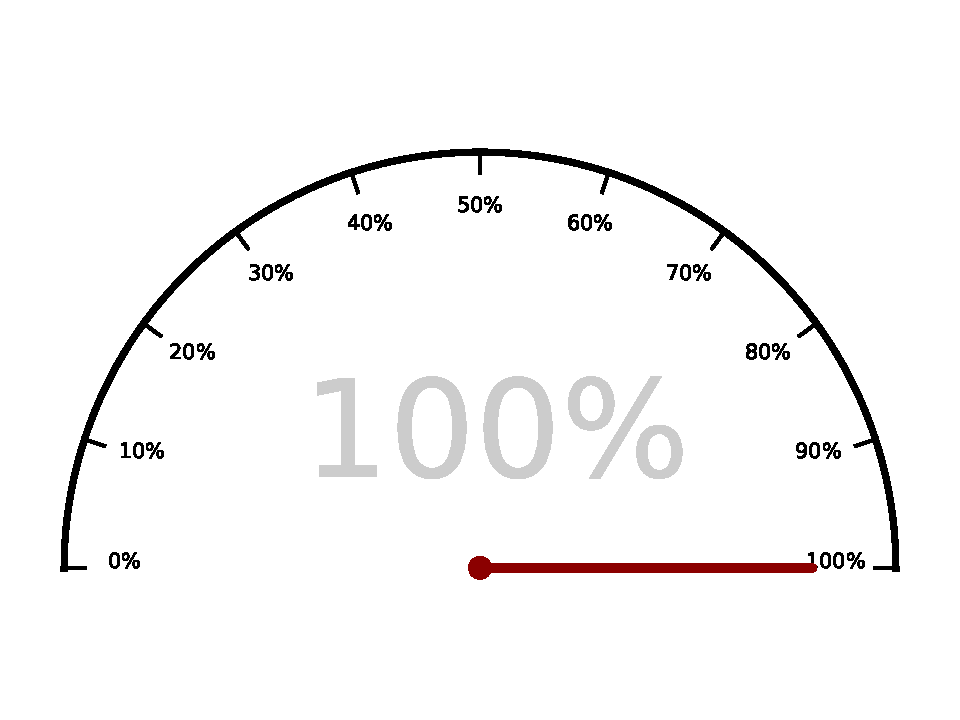
\includegraphics[width = .75\textwidth]{figures/poetryplots/speedometer.pdf}
\end{center}

You might prefer to make further modifications to the sizing and spacing depending. Below, we see some crowding with the tick labels. 

\pyfile{speedometers.py}

\begin{center}
    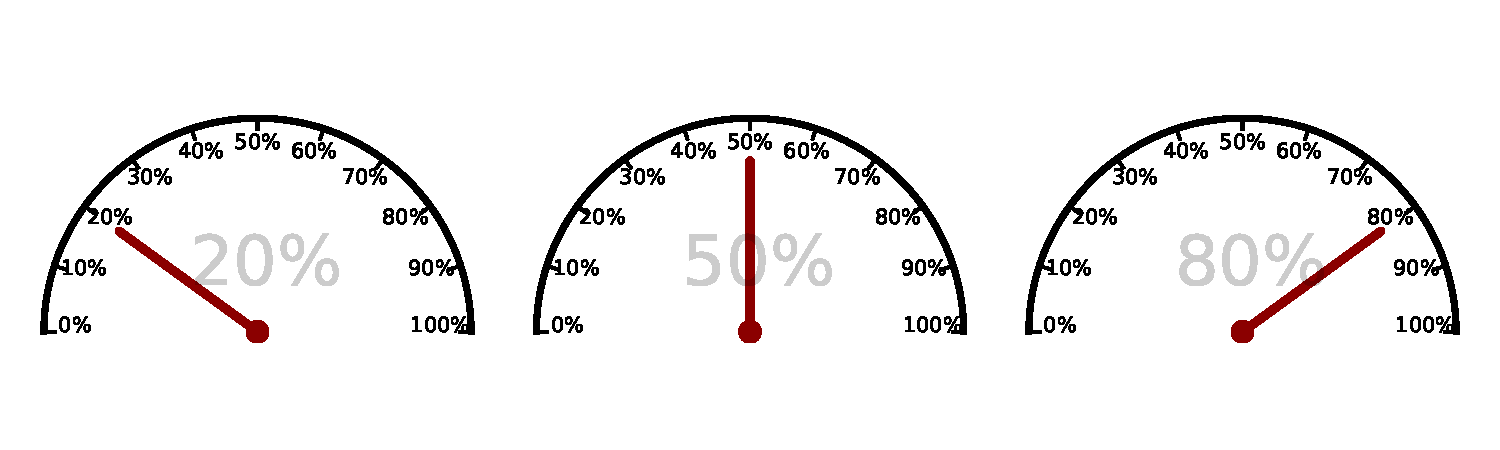
\includegraphics[width = .75\textwidth]{figures/poetryplots/speedometers.pdf}
\end{center}